\section{Results and Measurement Analysis}
\label{sec:experiments}

\subsection{Protocol}
The primary archive contains the first intra frame of 53 CTC sequences at
QP values $\{0,16,32,48,63\}$, giving 265 frame--QP pairs. We evaluate the
pinned e15 shared-latent checkpoint and one fixed router checkpoint at six
target budgets between 0.05 and 0.5\,dB. Reconstructions were produced by the
mixed tiled decoder; this revision reanalyses those outputs and does not
introduce new GPU measurements. Means compare the common cases for which
all four rules returned a plan. This leaves 204 pairs at 0.05\,dB,
263 at 0.1\,dB and 265 at each larger target. Missing plans are not silently
treated as successful full-depth fallbacks.

Paired confidence intervals resample sequences with all their available QPs
kept together, using 5,000 bootstrap draws. They describe variation over the
available content at fixed trained weights, not training-seed uncertainty.
We also repeat the budget trend on the same 204 pairs throughout to expose
the effect of changing cohort membership.

\subsection{The incremental value of content prediction}
At a 0.1\,dB target, source-informed search saves
\MainOracleSaving\% of modelled decoder MACs, the router
\MainRouterSaving\%, Bayer dithering \MainDitherSaving\%, and uniform depth
\MainUniformSaving\% (\cref{fig:budget}). The router's paired advantage over
dithering is \MainPremium\ points, with a 95\% interval of
[\MainPremiumLow, \MainPremiumHigh]. This is the incremental arithmetic value
of learned allocation under the recorded calibration procedure, not the
router's total saving against full depth.

The advantage declines as the target relaxes: it is \MediumPremium\ points
at 0.2\,dB, \LoosePremium\ at 0.3\,dB and \SaturatedPremium\ at 0.5\,dB.
The cheapest reachable exit imposes a \MacCeiling\% ceiling on this cost
model. Near that ceiling, many maps assign almost every tile to the same
exit, leaving little decision value for a content predictor. The fixed-cohort
analysis retains the declining trend, and the QP breakdown shows that its
location depends on the operating rate.

A fixed-histogram diagnostic isolates spatial placement further. For each
recorded map, we compute the exact expected table MSE after uniformly
permuting its exit assignments. This preserves the number of tiles at every
depth and hence its modelled cost. At 0.1\,dB, the router's placement improves
the table statistic by 0.0213\,dB on average (95\% interval
[0.0167, 0.0262]), while dithering gives 0.0007\,dB
([$-0.0002$, 0.0017]). These are source-table diagnostics, with the derivation
and fixed-histogram optimum in the supplement; final mixed reconstructions
would need to be decoded separately.

\begin{figure*}[t]
\centering
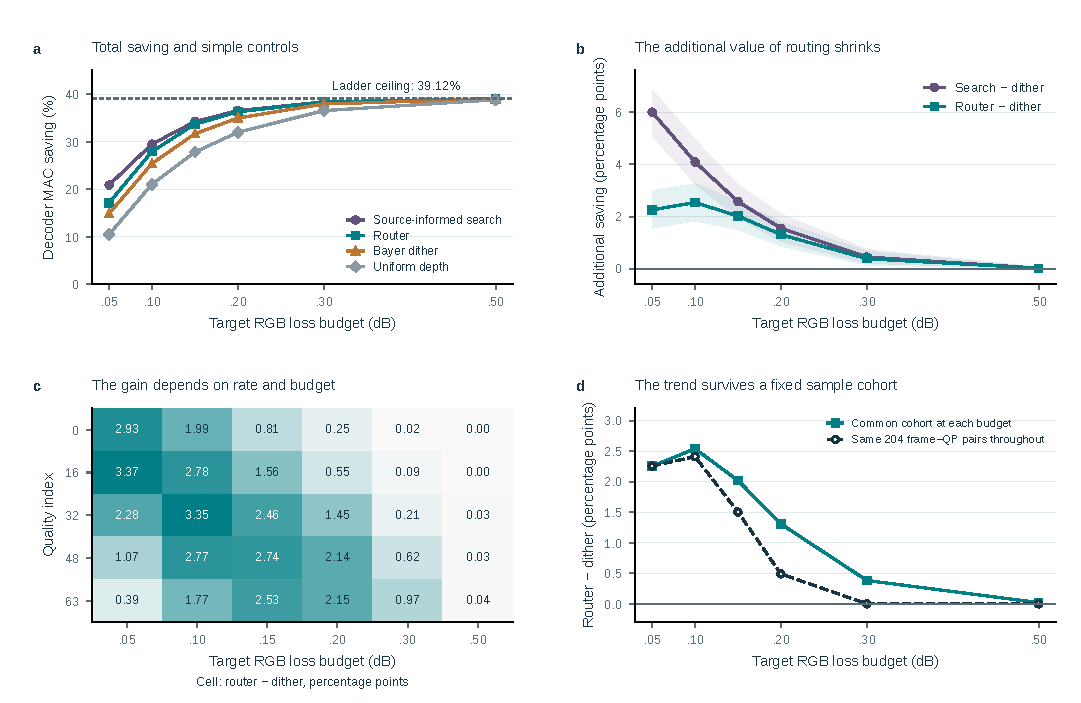
\includegraphics[width=\textwidth]{figs/refresh20260927/fig2_budget_value.pdf}
\caption{\textbf{Separate total saving from the value of routing.}
\textbf{a}, Four policies on their common cases at each target.
\textbf{b}, Paired differences with 95\% sequence-cluster bootstrap intervals.
\textbf{c}, Router--dither difference by QP and target, in percentage points.
\textbf{d}, The same comparison on a fixed cohort of 204 frame--QP pairs.
All curves use source-calibrated per-frame controls and a decoder MAC model;
they do not include router/signalling cost or constitute latency measurements.}
\label{fig:budget}
\end{figure*}

\subsection{A quality target is not a delivered guarantee}
The policies do not achieve exactly the same loss at the same nominal target
(\cref{fig:quality}a). At 0.1\,dB, the router exceeds target plus
$10^{-4}$\,dB in \MainRgbOver/\MainN\ cases in RGB and
\MainYuvOver/\MainN\ cases in YUV 6:1:1. Maximum losses are
\MainRgbMax\,dB and \MainYuvMax\,dB, respectively. These are crossings of the nominal numeric target in the exported metric,
not a clean test of a common-reference constraint: selection uses a released
anchor on padded RGB, while reporting uses the fine-tuned full-depth output
on cropped images. Metric choice and cross-tile coupling are additional
differences. The exported records cannot separate their contributions.
A framewise guarantee requires the same anchor, support and metric in
selection and final verification.

\begin{figure*}[t]
\centering
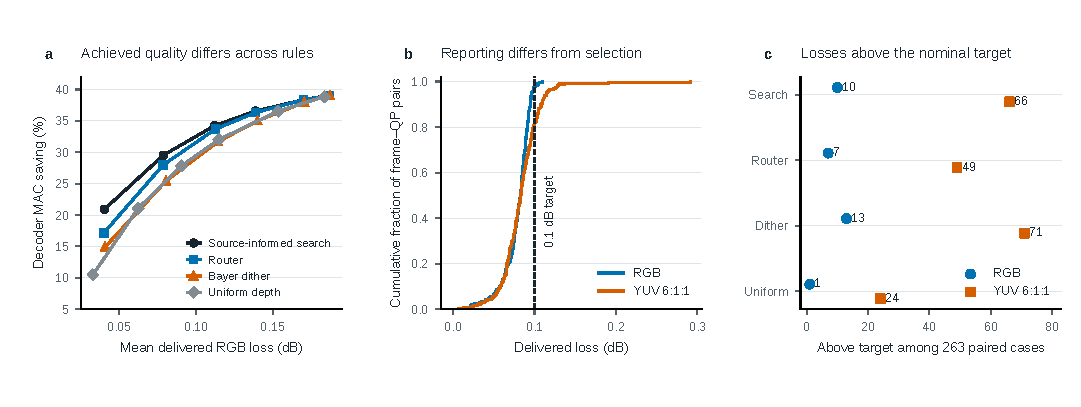
\includegraphics[width=\textwidth]{figs/refresh20260927/fig3_delivered_quality.pdf}
\caption{\textbf{Measure the reconstruction that is delivered.}
\textbf{a}, Recorded mean RGB loss against MAC saving; connected segments
guide the eye. \textbf{b}, Empirical loss distributions for the router at a
0.1\,dB target. \textbf{c}, Losses above the nominal target among 263 paired cases, measured
after cropping, with tolerance $10^{-4}$\,dB. The search used padded RGB
tables with a released-weight anchor; reporting uses the fine-tuned e15
full-depth anchor. Counts are not an isolated guarantee test. No verified
fallback was applied in this archive.}
\label{fig:quality}
\end{figure*}

\subsection{The encoder cost of knowing the source error}
The error table in \cref{eq:search} requires candidate reconstructions.
The historical QP32 benchmark recorded 1,347.65\,ms for six trial exits,
1,023.26\,ms after deduplicating the four reachable outputs, and 336.87\,ms
when a single tiled pass reused the common prefix (\cref{fig:decision}).
The last change reduces table-construction time by approximately fourfold.
These are the archived upper medians of 24 pooled trials over eight frames,
not an end-to-end encoder speedup. The raw repetition distribution and device
load history were not retained. Moreover, the archived GPU search timer can
include pending reference-decode work, so we do not use it as an isolated
search latency.

A fixed-control router can avoid the per-frame source-error table. The
source-calibrated router curves reported here cannot: they use that table to
choose $\beta$. A useful next comparison must therefore measure the complete
decision path under each information regime, including any extra stem work
at the encoder, map/control signalling and the final quality check.

\begin{figure*}[t]
\centering
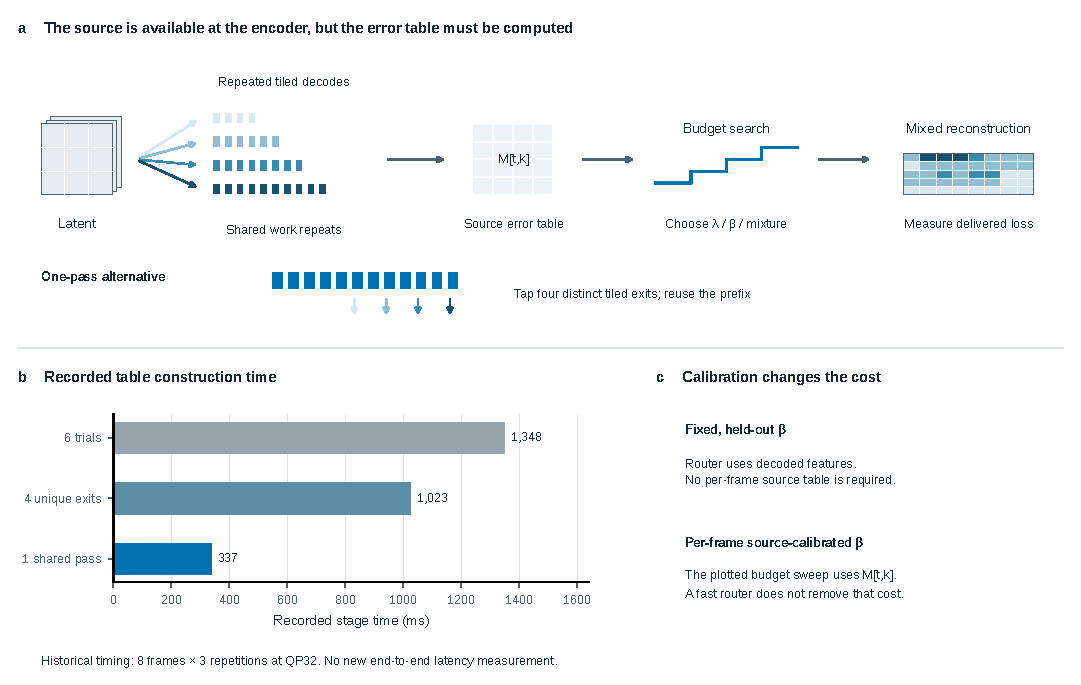
\includegraphics[width=\textwidth]{figs/refresh20260927/fig4_decision_cost.pdf}
\caption{\textbf{Obtaining the decision information has a cost.}
\textbf{a}, Candidate reconstruction, source-error tabulation, control search
and final mixed reconstruction are distinct stages. A shared pass can reuse
the trunk prefix. \textbf{b}, Archived table-construction timings; no raw
trial uncertainty is available. \textbf{c}, Fixed held-out control and
per-frame source calibration have different information requirements.
These historical stage measurements do not establish current end-to-end latency.}
\label{fig:decision}
\end{figure*}

\subsection{Spatial assignments and transfer limits}
\Cref{fig:maps} shows the recorded maps of one QP32 frame at two targets.
The example is chosen from the five archived thumbnails by proximity to the
aggregate router--dither premium at 0.1\,dB. The source thumbnail supplies
spatial context; it is not presented as a reconstruction-quality comparison.
The convergence of maps at the relaxed target illustrates the ladder's
saturation, but the aggregate claim comes from the full paired analysis.

\begin{figure*}[t]
\centering
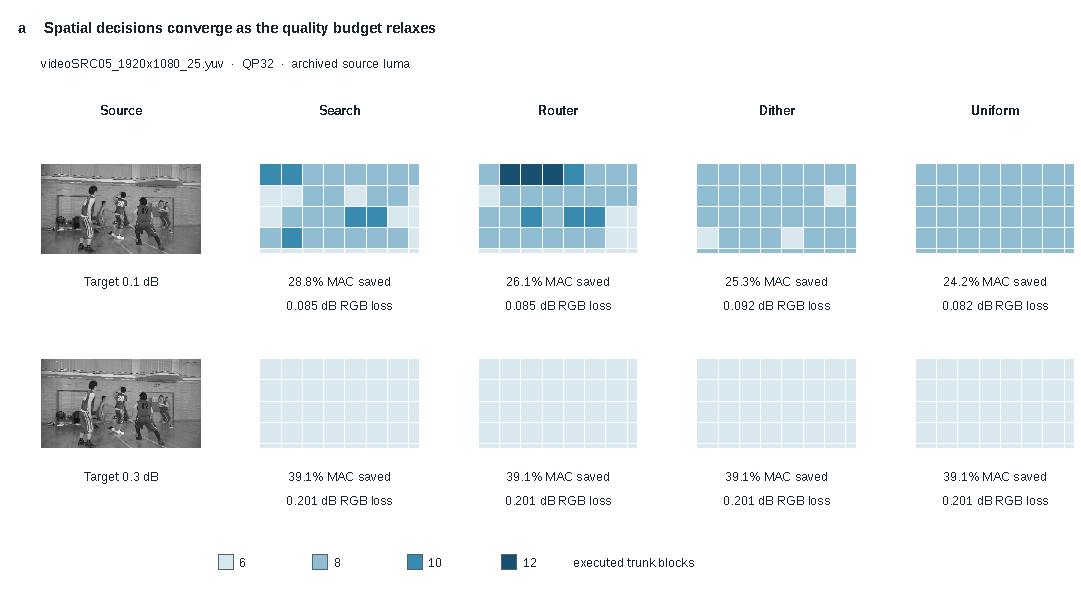
\includegraphics[width=\textwidth]{figs/refresh20260927/fig5_spatial_decisions.pdf}
\caption{\textbf{Recorded spatial decisions under two budgets.}
The left column is source luma. Other columns show actual maps, cropped to
the visible image extent, with executed depth, modelled MAC saving and
delivered RGB loss. This figure visualises allocation rather than perceptual
equivalence. The example-selection rule is stated in the text.}
\label{fig:maps}
\end{figure*}

Archived experiments on other decoders provide a useful boundary check
(\cref{fig:transfer}). Their selection criterion measures deviation from a
reference reconstruction, and their region/halo accounting models potential
compute reductions. The dense masked implementation evaluates candidates
before selection; these results therefore do not demonstrate conditional
execution speedups. The source-informed heuristic does not uniformly beat
the best blind control. Separate Kodak perceptual-budget experiments also
show that a PSNR constraint can permit appreciable LPIPS degradation.
Neither finding can be transferred into a numerical claim about DCVC-UF
without a matched experiment.

\begin{figure*}[t]
\centering
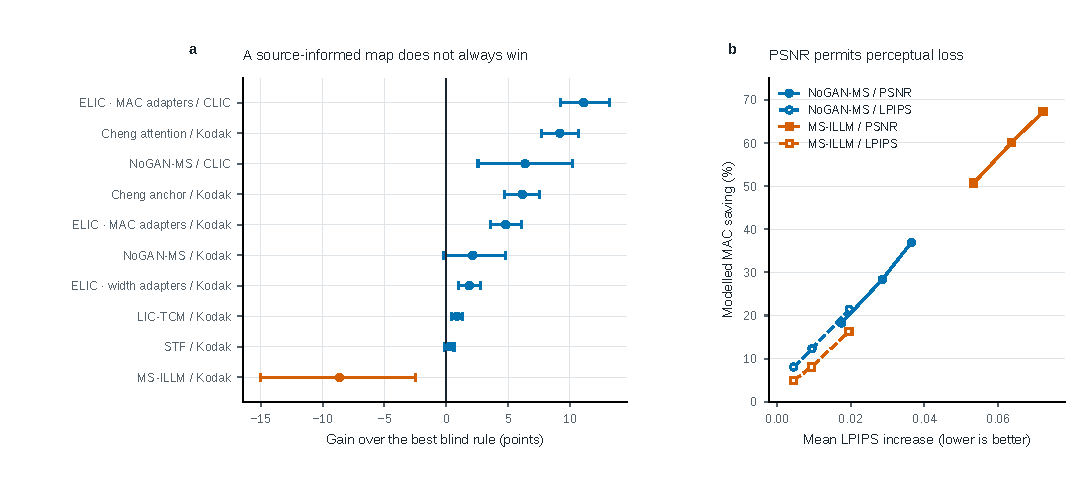
\includegraphics[width=\textwidth]{figs/refresh20260927/fig6_scope_and_perception.pdf}
\caption{\textbf{Architecture and metric limit the scope of the result.}
\textbf{a}, Source-informed selection minus the best dataset-level blind
rule at a 0.1\,dB target, with paired image-bootstrap 95\% intervals.
Adapter variants and datasets remain separate. Savings are modelled over
dense masked reconstructions. \textbf{b}, Independent Kodak-24 evaluations
under PSNR or LPIPS constraints for NoGAN-MS and MS-ILLM. The three points
per curve are recorded operating points, not interpolated observations.
These experiments use other decoders and do not validate FLEX latency or perception.}
\label{fig:transfer}
\end{figure*}
